This panel is where the user defines the structural model of the
building. The structural model is that part of the building provided
to resist the lateral loads. There are a number of backend
applications provided for this part of the workflow, each responsible
for providing the structural analysis model to the workflow. The
drop-down menu at the top of this panel is where the user selects
which application to use. As the user switches between applications,
the entry data changes to reflect the different inputs the different
applications require. At present there are two backend applications
available through the drop down menu: Multiple Degrees of Freedom
(MDOF) and OpenSees.

\subsection{Multiple Degrees of Freedom (MDOF)}

This panel is provided for users to quickly create simple shear models
of a building. The panel, as shown in \autoref{fig:mdof} is divided
into 3 frames:
\begin{enumerate}
\item in the top left frame the user enters the number of stories. For
  each story the user then enter the story height, initial stifness in
  1 and 2 directions, yield strength in 1 and 2 directions, and
  hardeing ratio again in 1 and 2 directions. In addition user enters
  the floor weights and damping ratios for each of the modes.
\item In the lower left frame the user has the option of overriding an
  an individual floor or story basis, any of the properties set in the
  upper frame.
\item on the right side of the frame is a graphical widget showing the
  current building. When entering data into the lower left frame,
  those floors and stories corresponding to data being modified is
  highlighted in red.
\end{enumerate}

\begin{figure}[!htbp]
  \centering {
    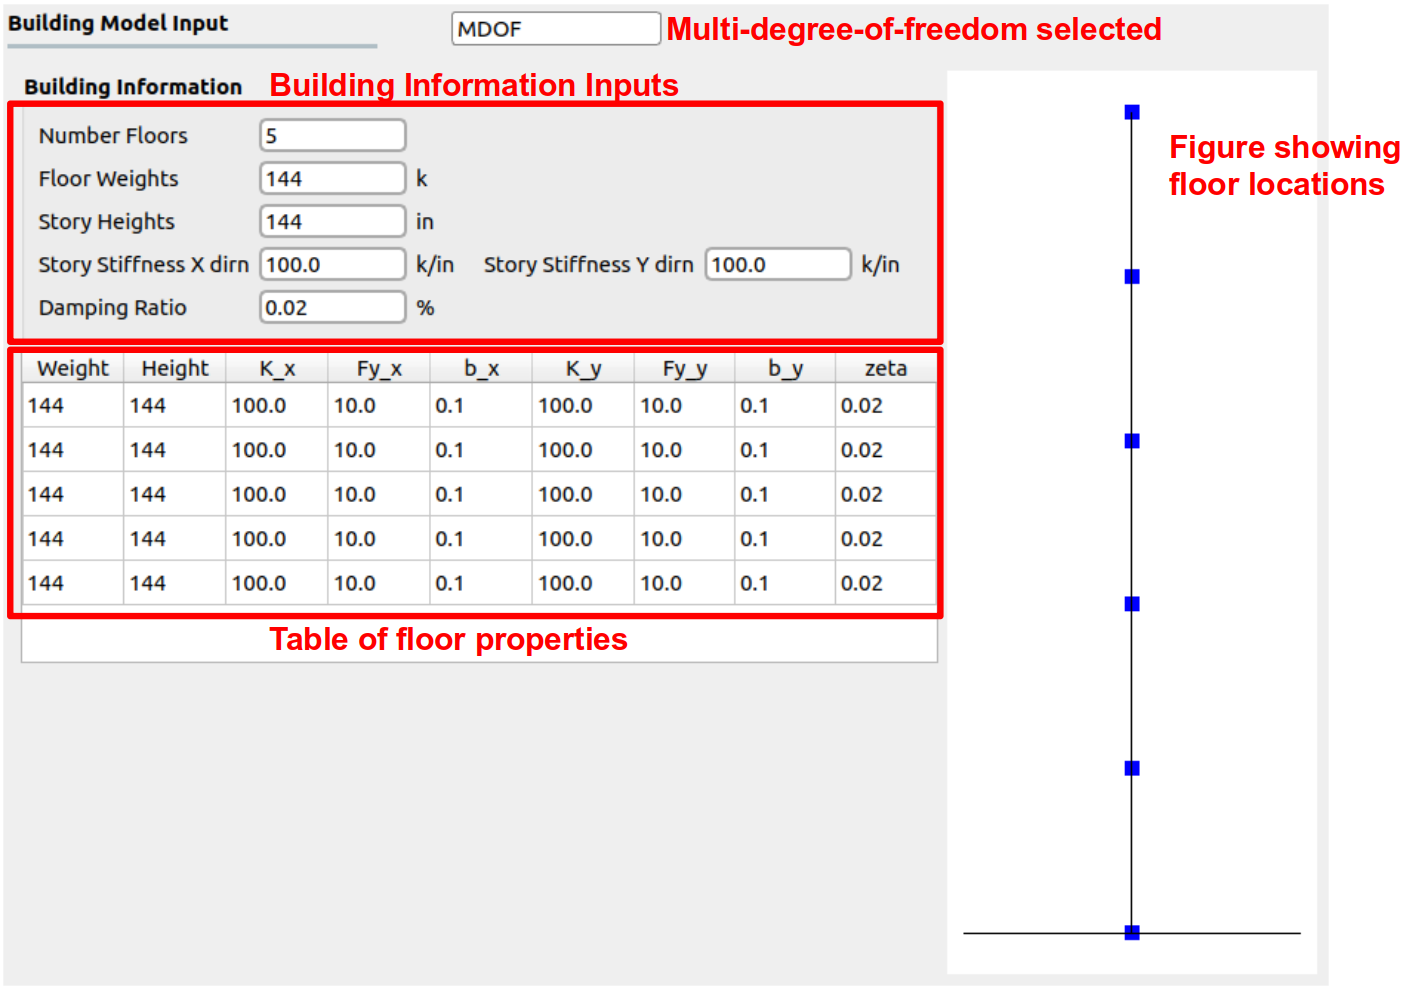
\includegraphics[width=0.8\textwidth]
    {usage/figures/mdof.png} }
  \caption{MDOF Model Definition}
  \label{fig:mdof}
\end{figure}

Random Variables: Random Variables can be created by the user entering
a valid string instead of a number in the entry fields for all entries
except the number of floors. The variable name entered will appear as
a Random Variable in the UQ panel and it is there that the user must
enter the distribution for the Random Variable.


\subsection{OpenSees}
The panel is for users who have existing OpenSees model of a building
that performs a gravity analysis and now wish to subject that building
model to one of the EVENT options provided. The panel that presents is
as shown in \autoref{fig:figure3}. The user has 3 fields that he needs
to fill out:
\begin{enumerate} 
\item The user specifies the main script that contains the building
  model. This script should build a model and perform any gravity
  analysis of the building that is required before the event is
  applied.
\item A llist of nodes that define a column line of interest for which
  the responses will be determined. The column nodes should be in
  order from ground floor through to roof. The EDP options use this
  information to determine nodes at which displacement, acceleration
  and story drifts are calculated.
\item An entry for the dimension of the model, i.e. 1D, 2D or 3D. This
  information is used to apply ground motions.
\end{enumerate}

\begin{figure}[!htbp]
  \centering {
    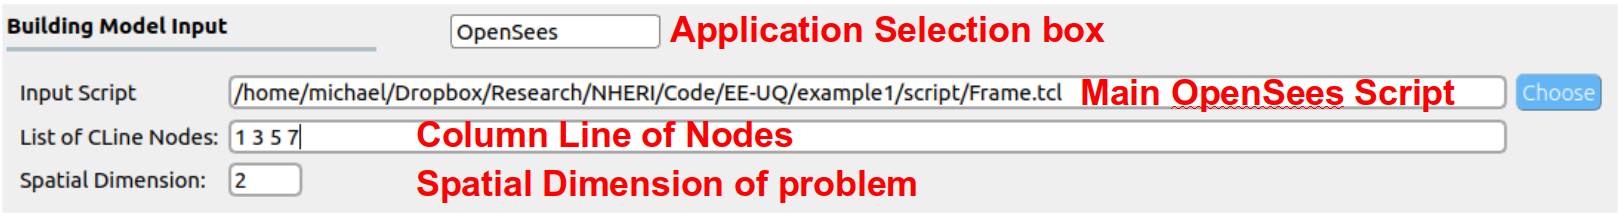
\includegraphics[width=0.8\textwidth]
    {usage/figures/openSees.png} }
  \caption{OpenSees Input Model}
  \label{fig:figure3}
\end{figure}

Random Variables: In OpenSees there is an option to set variables to
have certain values using the pset command, e.g pset a 5.0 will set
the variable a to have a value 5 in an OpenSees script. In EE-UQ any
variable found in the main script to be set using the pset command
will be assumed to be a Random Variable. As such, when a new main
script is loaded all variables set with pset will appear as Random
Variables in the UQ panel.
